\chapter{Research Description}
\label{sec:researchdesc} 

\section{Introduction}
\label{sec:introduction}

\section{Background of the Study}
\label{sec:backgroundstudy}

% What is NA Quantification and its applications ? %
Detection of target molecules found in deoxyribonucleic acid (DNA) or ribonucleic acid (RNA) is a rapidly growing field of study in the interest of quantifying gene expression levels \cite{Huggett2015_PCR_NGS}. These nucleic acid strands carry genetic information and are used as biomarkers for the detection of diseases. Additionally, along with the rise of bioinformatics tools, quantification methods are also utilized in rare mutation detection, copy number variation detection, single-cell gene and microRNA expression analysis, and next-generation sequencing \cite{Quan2018}. Outside the scope of molecular biology, its application has also found its way in forensic research \cite{Whale2013}, medical diagnosis, environmental monitoring, and food safety analysis \cite{Cao2017}.

% TODO : Brief history of dPCR (3 sentences ) %
% TODO : What is the difference of qPCR with dPCR (2 sentences) %

% How to Quantify NA Quantification with (dPRC) ? %
Before target molecules can be quantified, the challenge of detecting these microscopic targets should be addressed first. In a DNA sample, the relative concentration of target DNA is undetectably low. One solution to this problem is to amplify the DNA sequences using polymerase chain reaction (PCR), a widely-used method for nucleic acid amplification since its invention in the 1980s \cite{Cao2017}. PCR exponentially multiplies specific targets in the DNA or cDNA strands into millions to billions of copies (Figure \ref{fig:pcr_explained} (A)). The dPCR sample preparation consists of mixing the DNA sample with chemical components that will encourage the amplification, such as buffers, Taq polymerase, and intercalating dyes or fluorescence probes. This blend of chemicals, called the reaction mix, is pipetted into an assay containing equal sized reaction wells, thereby partitioning the reaction mix into thousands of droplets (Figure \ref{fig:pcr_explained} (B)). The assay is then exposed in a series of 20 to 40 thermal cycles. In each cycle, the process of denaturation, annealing, and extension are performed which doubles the target DNA copy -- theoretically producing \(2^n\) molecules after \(n\) cycles \cite{Quan2018}. A droplet that contains at least one target DNA copy will emit high fluorescence intensity; each droplet is then "digitized", or classified binarily as "positive" or "negative", based on its fluorescence amplitude (Figure \ref{fig:pcr_explained} (C)).

\begin{figure}[h]
    \centering
    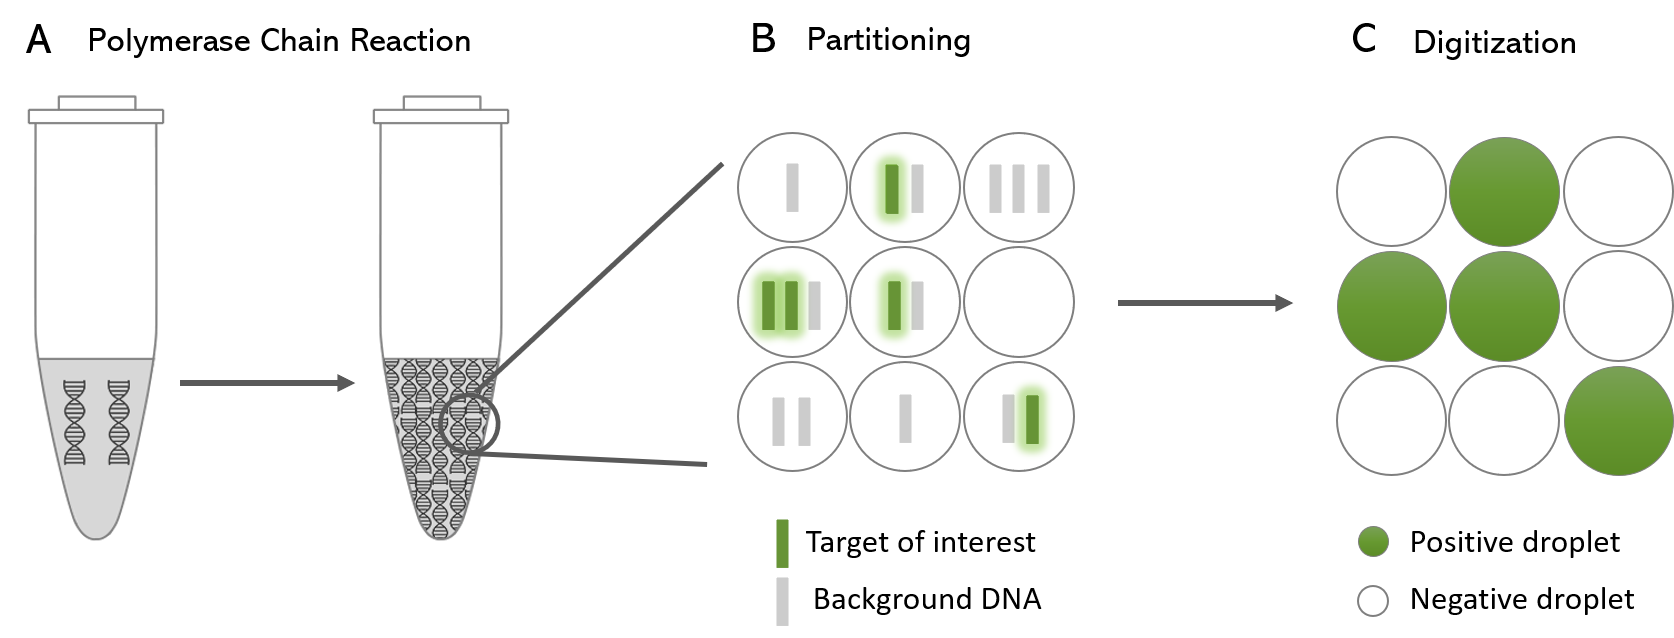
\includegraphics[max size={\textwidth}{\textheight}]{pcr_explained.png}
    \caption[Digital PCR Quantification Steps]{Digital PCR Quantification Steps}
        \label{fig:pcr_explained}
\end{figure}

% What are the advantages of dPCR? %
Since the earliest published dPCR experiment from 1988 (\citeauthor{Saiki1988}), the advances of nanofluidic technology in biomedical instruments have continuously pushed the limits of dPCR. An increasing number of researchers have found dPCR to be reaching, and even outperforming, the precision, sensitivity, and reproducibility of real-time qPCR, which is the gold standard for molecular quantification \cite{Chen2018, Persson2018, Taylor2017, Arvia2017, Blaya2016, Jones2016, Sanders2011}. The nature of dPCR allows it to standardize quantitation as opposed to qPCR's use of a reference curve, resistant to inhibition, and less negatively influenced by the target sequence variability \cite{Sedlak2014}. The unraveling superiority of dPCR makes it a necessity for research experiments that require intensive accuracy, such as the certification or stability studies of reference materials.

% - GMO - Because of regulation of cultivation and trade of GMOs in several countries, there is pressure for their accurate detection and quantification. Today, DNA-based approaches are more popular for this purpose than protein-based methods, and real-time quantitative PCR (qPCR) is still the gold standard in GMO analytics. However, digital PCR (dPCR) offers several advantages over qPCR, making this new technique appealing also for GMO analysis. (Demeke) %
% - circRnucleic acid - Diagnostics based on circulating circular RNA (circRNA) is an emerging field for noninvasive molecular diagnosis, owing to the stable circular structure of circRNA. However, CircRNA remains stable in the promptly separated serum/plasma within 24 h and is a promising candidate for biomarker research. In addition, because the concentration of circRNA will be affected if the clotted blood and EDTA blood are not centrifuged promptly, samples should be handed in a timely manner to reduce the hematocyte-derived varia- tion. (Chen, DF) %

% What are the current challenges in dPCR experiments? %
Despite the optimistic performance of dPCR, several challenges are met before being able to reach the optimal results from dPCR. One of the final steps in dPCR is the threshold determination that separates the endpoint fluorescence of the dPCR assay into positives and negatives. This threshold is not constant for all DNA samples and is unclear for assays that produce ambiguous readouts \cite{Trypsteen2015}.

An important aspect of positioning the threshold is the presence of noise features in the data. Poor quality dPCR assays add to the ambiguity of fluorescence signals that contribute to the difficulty of threshold determination. Due to the emerging demand for dPCR data analysis, \citeA{Lievens2016} has determined a set of method performance criteria to assess the quality of a dPCR assay run. Their following criteria aims to measure the efficiency of the separation between positive and negative droplets: (i) there should only be two fluorescence populations, or in other terms, a single amplification product; (ii) there should be a good separation between positives and negatives measured in peak resolution; and (iii) there should be very minimal amounts of intermediate fluorescence, also called as 'rain'. The factors affecting these noise characteristics are further explored in the succeeding sections. 

``Rain" is the term used in several studies to describe droplets that emits a fluorescence intensity settling in between the positive and negative populations \cite{Lievens2016, Trypsteen2015, Witte2016, Dreo2014, Brink2018, Attali2016}. Figures \ref{fig:plate1cru} and \ref{fig:plate1tc1507} demonstrate two different DNA targets with the former showing a visually clearer distinction of the positive and negative population than the latter, of which is possessing multiple rain droplets. The data used in these figures are sourced from the dataset made publicly available by \shortciteA{Lievens2016}. Having more than two fluorescence population is also a problem, since it is not known whether these droplets do contain the target DNA or are just fluorescence residue. Poor quality dPCR assays negatively limit the level of sensitivity and accuracy it may reach. Among the consequences of unoptimized dPCR assays is droplet misclassification, which may lead to serious misdiagnoses.

\begin{figure}[h]
    \centering
    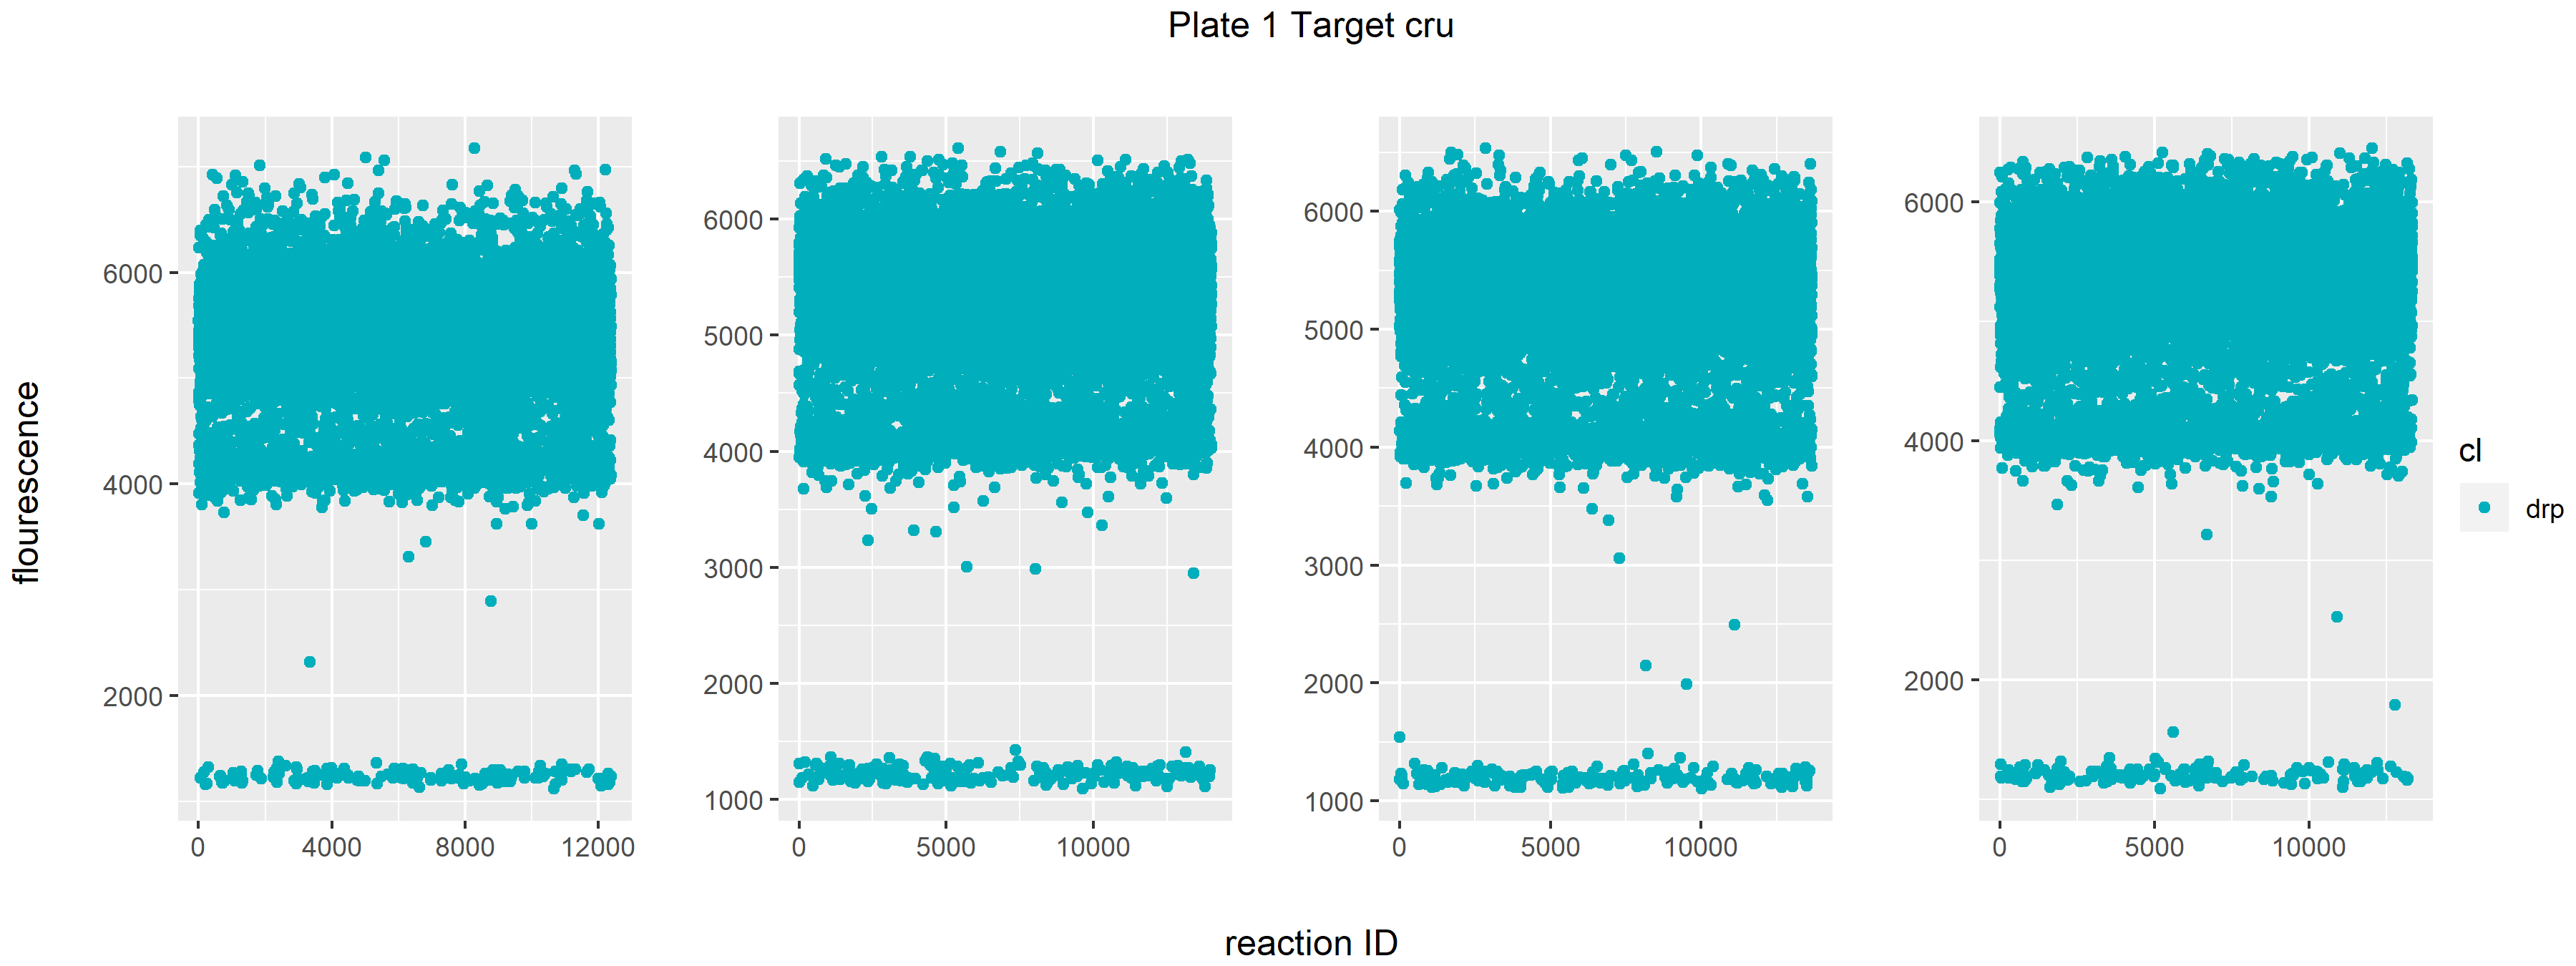
\includegraphics[max size={\textwidth}{\textheight}]{Plate 1 Target cru.png}
    \caption{Fluorescence readings of 4 repititions of DNA target cru}
        \label{fig:plate1cru}
\end{figure}

\begin{figure}[h]
    \centering
    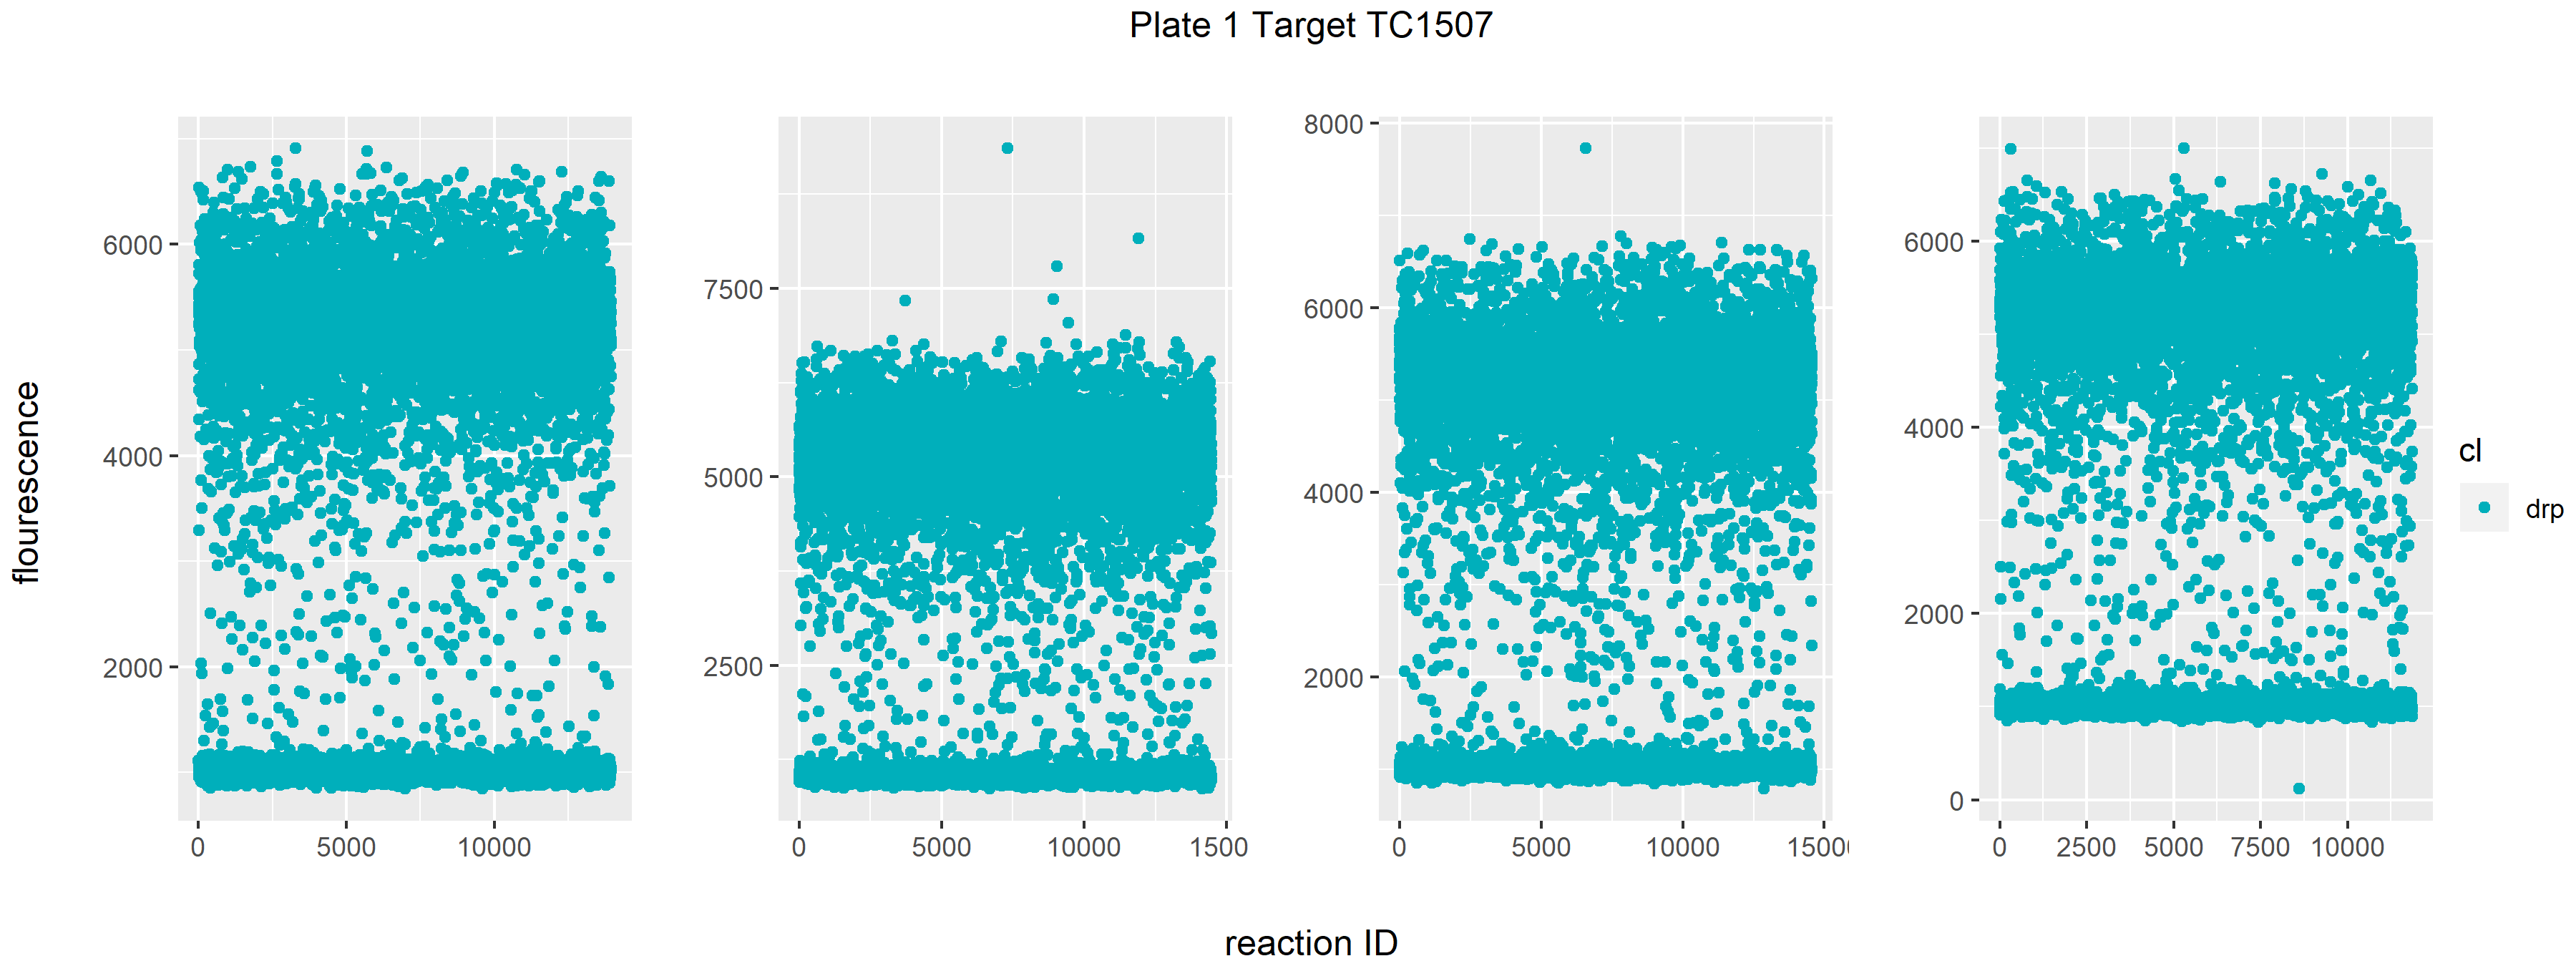
\includegraphics[max size={\textwidth}{\textheight}]{Plate 1 Target TC1507.png}
    \caption{Fluorescence readings of 4 repititions of DNA target TC1507}
        \label{fig:plate1tc1507}
\end{figure}

Estimating the DNA target concentration is based on the classification of positive and negative droplets. When assays produce two distant fluorescence populations, most quantification tools can estimate target concentrations with high sensitivity. As demonstrated in an optimized E. amylovora experiment \cite{Dreo2014}, slight differences of thresholds calculated from different tools had little effect on the final estimated concentration. However, for R. solanacearum, which is observed to manifest false-positive signals in qPCR experiments, produced unsatisfactory analytical sensitivity of the concentration estimates. The danger of low sensitivity is expounded at the clinical level, where inaccurate target quantification leads to the misdiagnosis of patients \cite{Tzonev2018}. One such case is the prenatal screening test for Down Syndrome; this test is expected to mostly result in normal pregnancies. However, many pregnancies are still falsely reported as positive for Down Syndrome. False negatives also risk the overall health of the patient that truly possesses the genetic disorder.

% Important variance components are included as arrows between the appropriate steps. The steps are: (1) extracting RNA or DNA from the biological sample, (2) preparing the PCR master mix and including a quantity of extract, (3) dividing the reaction mix over a large number of partitions (droplets or cells), (4) amplifying the target material present in the partitions over a selected number of amplification cycles and measuring the endpoint fluorescence and (5) estimating the target concentration and quantifying the uncertainty on the estimates. Variance components are (i) technical variation: sampling variation and pipette error, (ii) machine-specific variation: unequal partition size and possible partition loss, and (iii) possibly user-optimized (mis)classification of endpoint fluorescence.

% What are the factors that cause these noise %
The whole dPCR workflow introduces multiple entry points for technical error, which may add "noise" in the amplified fluorescence. As illustrated in \figref{fig:dpcrWorkflow}, the workflow is usually a sequential procedure of extracting from a biological sample, preparing and partitioning the reaction mix, amplifying the assay, detecting the target molecules, and then finally, the target concentration is estimated using a Poisson correction factor. \citeA{Jacobs2014} emphasized that every step of the dPCR workflow inevitably allows for the introduction of different sources of variation shown in \figref{fig:dpcrWorkflow}. Operator-specific and repeatability variations are caused by pipetting skills, aliquot mismeasurements, and sample preparation time (when prolonged, probe degradation occurs which affects the quality of emitted fluorescence). Machine-specific variation may be caused by unequal partition sizes and possible partition loss. Finally, even if the former variations were managed, sample assay replicates such as in Figure \ref{fig:dpcrWorkflow}. B, will still produce varying target concentration estimates due to sampling errors. These errors are caused by 1.) sub-sampling only a portion of an organism and 2.) uneven counts of target copies distributed in the partitions. In addition to operator and machine variations, sample preparation in itself is a challenge as the optimal parameters in designing the reaction mix need to be identified. These parameters or experimental factors in Figure \ref{fig:pcrExperimentalFactors}. A affect the dPCR amplification efficiency. When these experimental factors are not optimal, assays generate ambiguous fluorescence readouts as shown in Figure \ref{fig:pcrExperimentalFactors}. B. It is not clear where to set the threshold that separates positive and negative droplets, in these scenarios, droplet misclassification error is prevalent.

\begin{figure}[h]
    \centering
    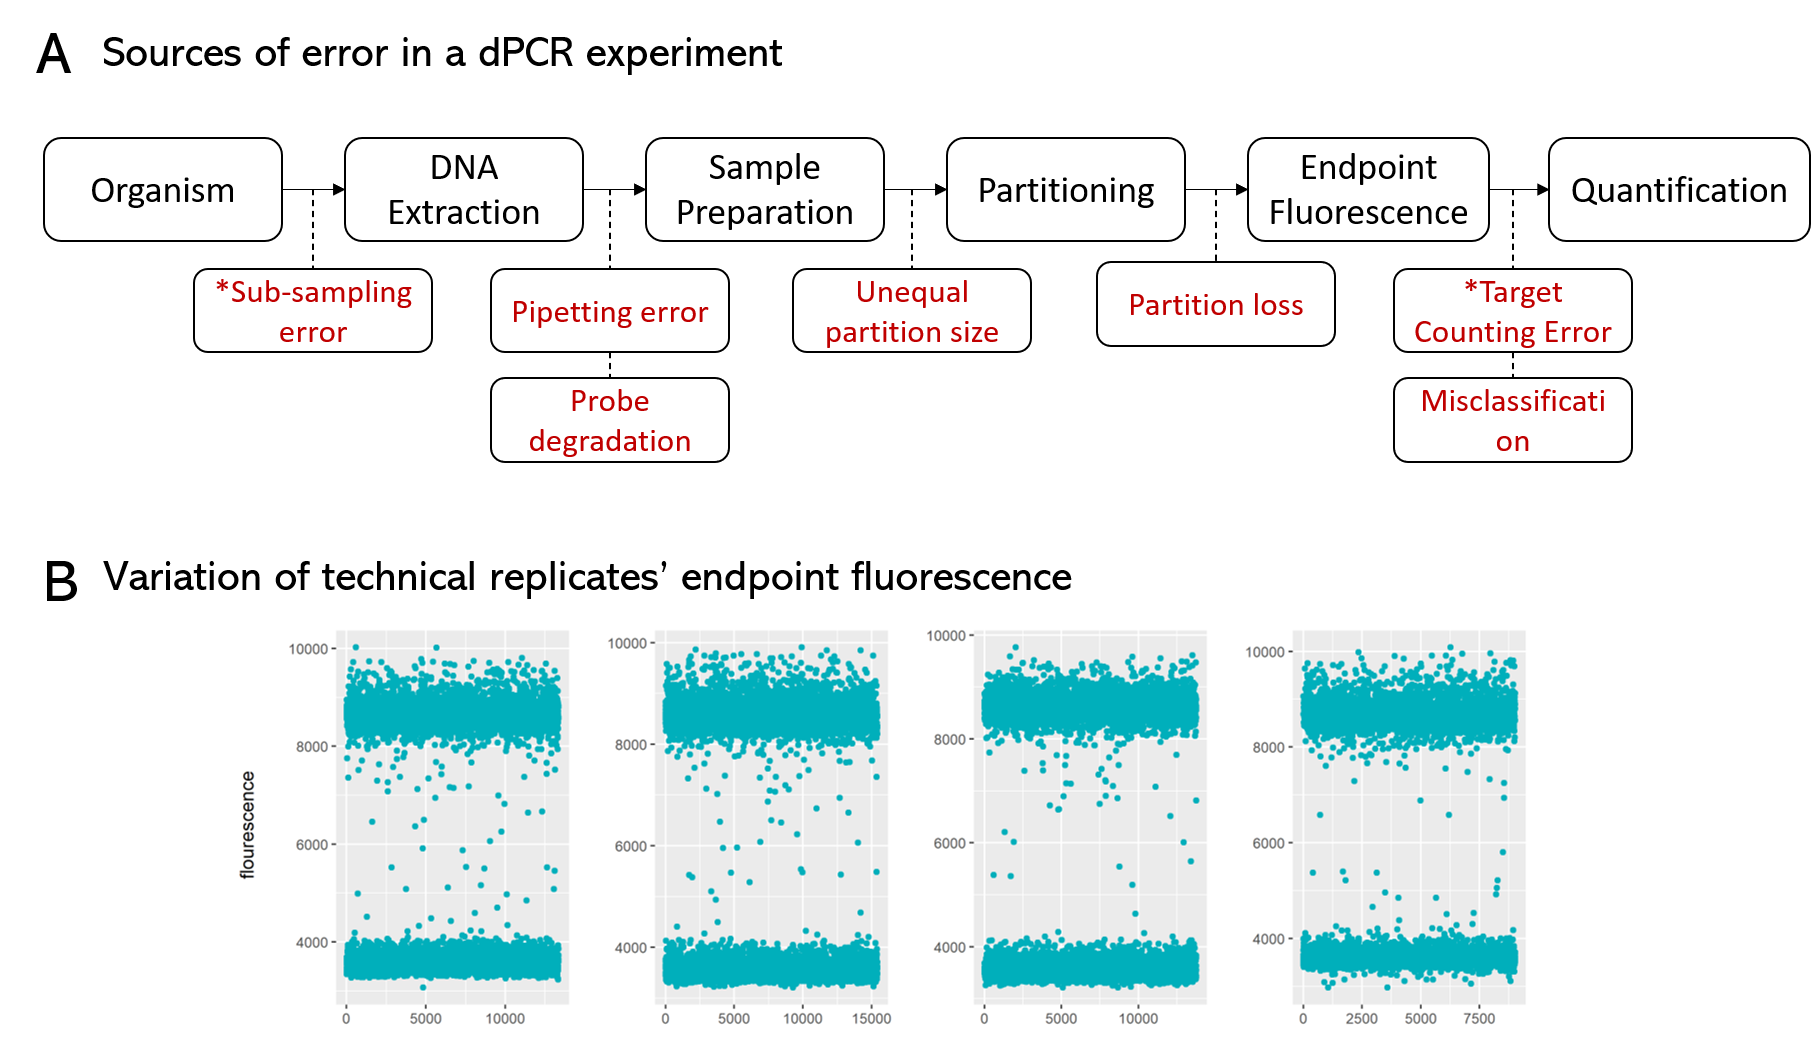
\includegraphics[max size={\textwidth}{\textheight}]{dpcrWorkflow.png}
    \caption[Sources of variation in the dPCR workflow]%
    {Sources of variation in the dPCR workflow- (A) Multiple sources of error can be introduced for each step in the dPCR workflow. Items with `*' indicate sampling error). (B) In effect, sample replicates obtained from the same organism will inevitably have variation in its fluorescence readouts. }
        \label{fig:dpcrWorkflow}
\end{figure}

\begin{figure}[h]
    \centering
    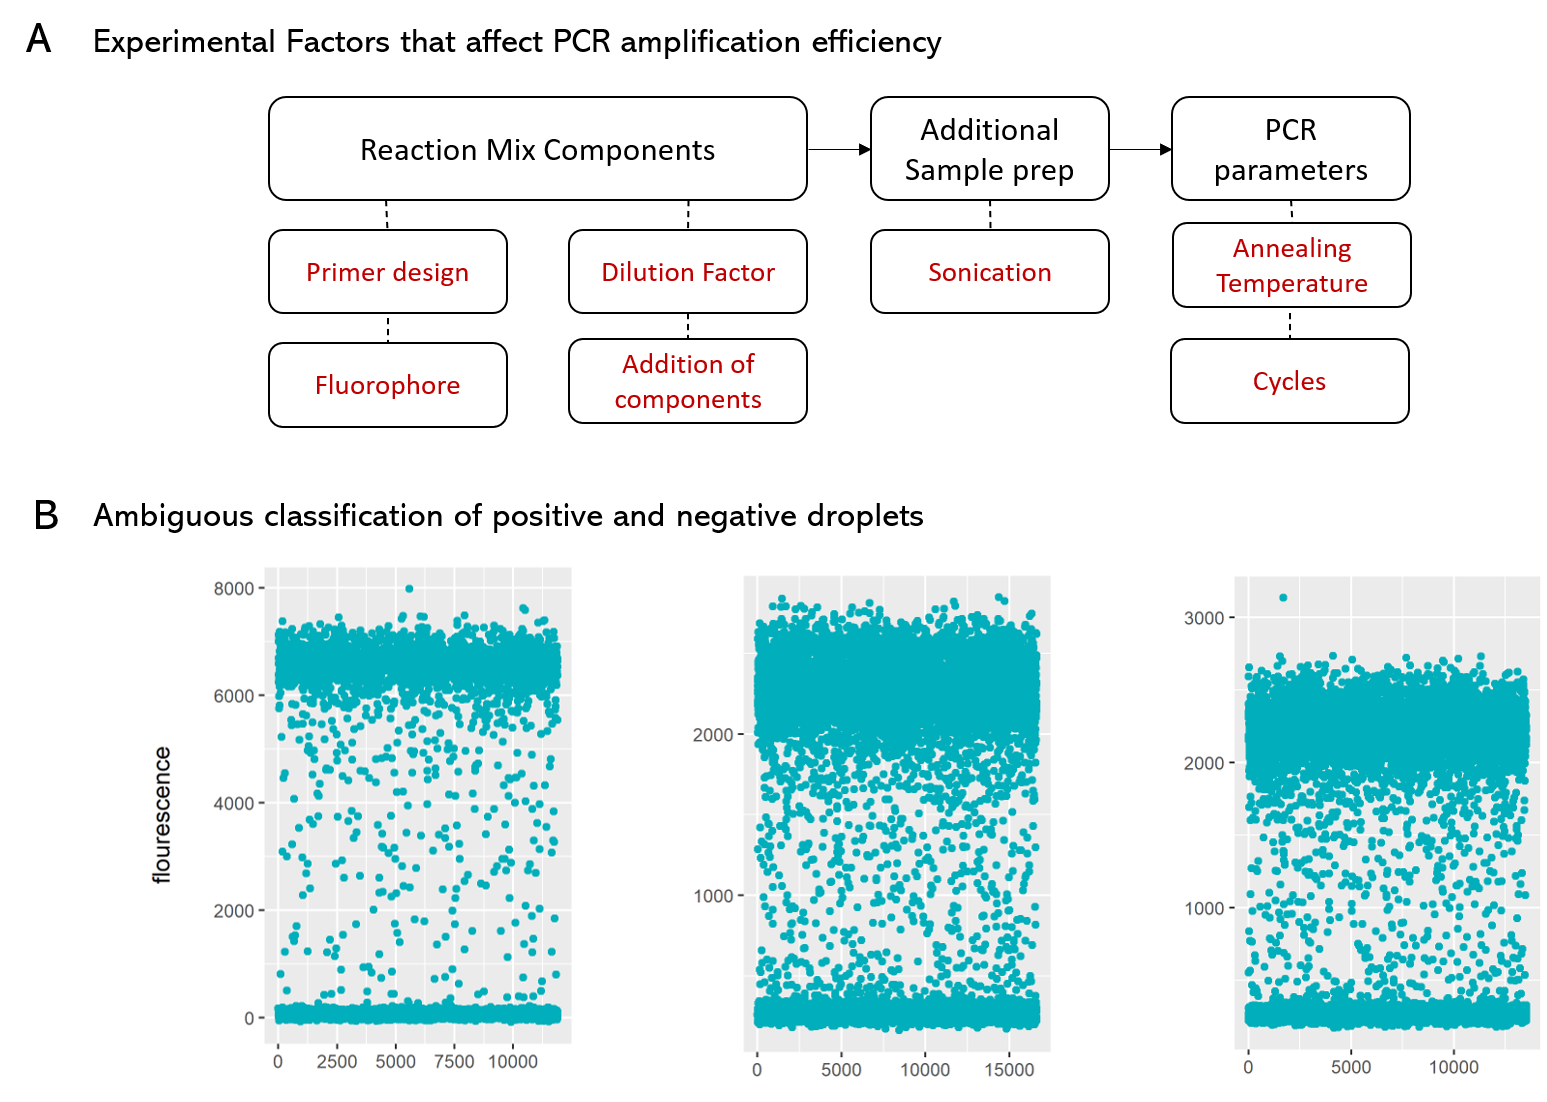
\includegraphics[max size={\textwidth}{\textheight}]{pcrExperimentalFactors.png}
    \caption[Experimental factors that affect dPCR amplification]%
    {Experimental factors that affect dPCR amplification- (A) List of parameters that may be controlled to optimize dPCR amplification (B) Unoptimized assays produce ambiguous readouts, making it difficult to determine a clear demarcation line between the positive and negative droplets }
        \label{fig:pcrExperimentalFactors}
\end{figure}

% Physical variations %
Different dPCR systems do not share a common default setting and thermal profiles. Each one is a factor that has to be optimized depending on the target molecule. Increasing the number of cycles has shown to affect the amplification of dPCR droplets that increases the separation of the two populations \cite{Koppel2015}. Temperature gradients are frequently performed to find the most favorable setting to reduce rain \cite{Gerdes2016}. However, the optimized parameters to improve the quality of a target's dPCR assay may not work for another target. As shown in the experiment of \shortciteA{Witte2016}, parameters that increased the efficiency for prfA did not work for \(\Delta\)prfA. Besides controllable settings, different dPCR platforms also have been revealed to deviate from its claimed volume \cite{Pinheiro2012,Dong2015,Corbisier2015,Dagata2016,Kosir2017}. These discrepancies have been observed in the Bio-Rad QX100/QX200 platforms and the RainDrop platform. Unequal partition volumes may produce suboptimal PCR amplification that contributes to increased rain droplets.

% Biological and Chemical variations % 
In addition to physical variation, chemical and biological factors play a role in the dPCR assay quality, such as target sequence variation, amount of polymerase, MgCI2, dNTPs, and primers \cite{Koppel2015, Kramer2001}, dye or probe quencher \cite{Witte2016}, fluorophore used \cite{Gerdes2016}, inhibition, delayed reactions, primer depletion, and other biological factors \cite{Jacobs2014}.

% Sampling variations %
Sampling variation stems from the fact that only a small sample of the organism is extracted; and although there is an expected number of target molecules per liters of a sample, drawing equally sized samples will result in different target molecules that are more or less near the average. \shortciteA{Tzonev2018} demonstrates the number of target molecules that can be drawn from extraction is distributed as Poisson. Besides the sampling error, samples may also exhibit imperfections, and thus have inhibited amplification. Each variance component accumulates to the bias and variance of the final estimated target concentration, and thus, this gives rise to the importance of providing solutions that would increase precision in every step. To increase the sensitivity and specificity of the estimate, the misclassification of droplet partition should be minimized as much as possible. A high presence of false-negative droplets reduces sensitivity, while specificity is lowered for high false-positive counts. 

% What can be done to reduce the noise indicated above? %
The factor directly causing noisy readouts is very difficult to pinpoint. In case of failure to optimize the design parameters, other hands-on approaches may be taken, such as running a real-time qPCR experiment, running PCR solution in gel electrophoresis, or performing dilution series in the cost of additional labor. However, preparing replicate samples are prone to pipetting and operator errors. On the other hand, the problem may also be alleviated using statistical approaches. For droplet volume variability, that means a correction-factor must be taken into account to improve the agreement of estimates. In the case of unoptimized assays, statistical methods can help automatically determine the threshold to separate the positive and negative droplets and also eliminate manual operator bias. Based on the experience of \citeA{Demeke2018}, they were able to produce precise estimates from unoptimized assays due to statistically-based thresholds. When dealing with rain, some researchers exclude it in the final droplet counts \cite{Jones2014}, but this option is said to produce underestimated concentrations if rain were actually suboptimal PCR reactions; instead, the threshold algorithm should be improved \cite{Trypsteen2015}. Based on expert opinion, rain droplets may also be caused by primer dimers, which are primers that annealed together instead of the target DNA. Because of the different interpretations of rain droplets, adjusting the threshold should be a feature available for droplet classifier systems.

\begin{figure}[h]
    \centering
    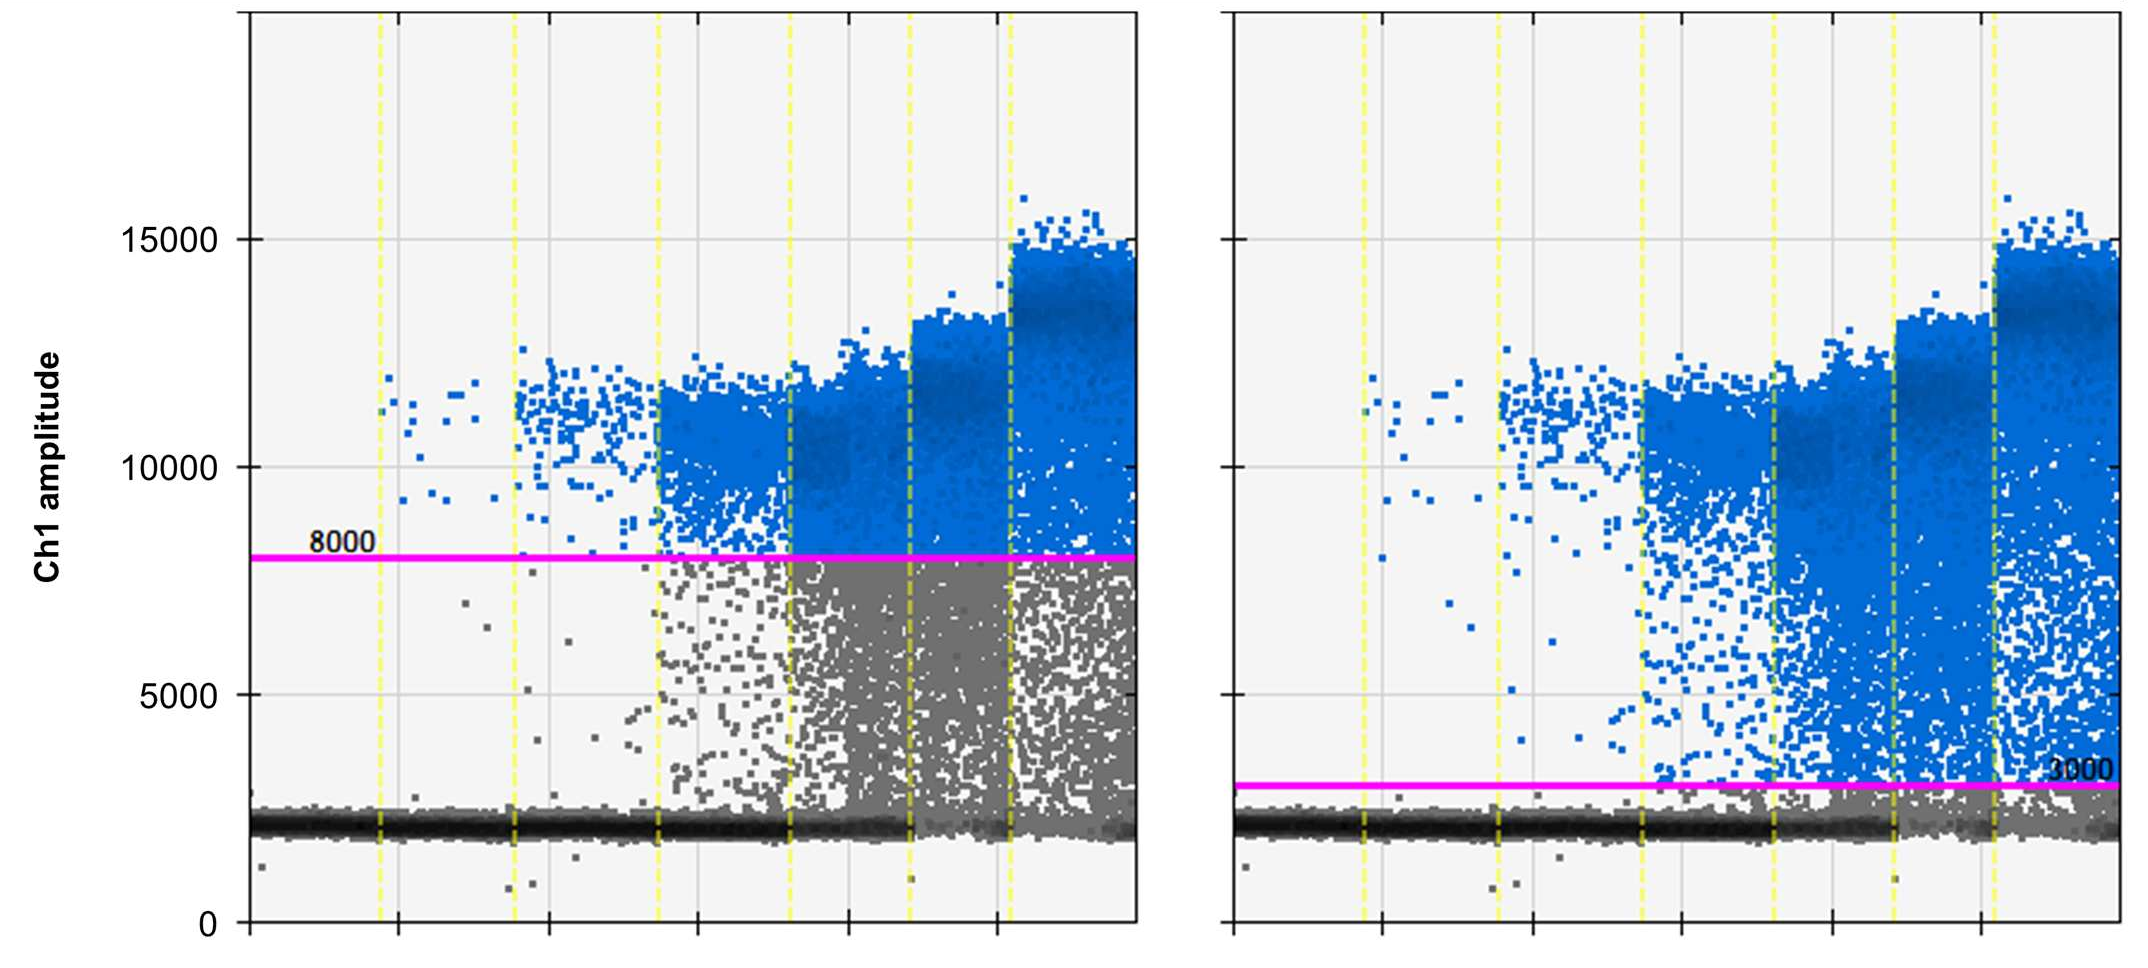
\includegraphics[max size={\textwidth}{\textheight}]{ambiguous_readouts.png}
    \caption[QuantaSoft High and Low Threshold Settings]{QuantaSoft High and Low Threshold Settings- Reprinted from "Systematic Investigation of Parameters Influencing Droplet Rain in the Listeria monocytogenes prfA Assay - Reduction of Ambiguous Results in ddPCR," by Witte, A. K., Mester, P., Fister, S., Witte, M., Schoder, D., \& Rossmanith, P., 2016, A PLOS ONE, 11(12), https://doi.org/10.1371/journal.pone.0168179}
        \label{fig:quantasoftThreshold}
\end{figure}

% A statistical approach is proposed in this study. %
Expounding further on the automated threshold setting approach, current algorithms can be improved and should be robust to baseline shifts, rain droplets, multiple populations, and poor separation of populations. The baseline fluorescence of the negative population has been observed, but even the popularly used QuantaSoft systems do not take this into account \cite{Trypsteen2015}. Thus, discrepancies may occur in the number of positive droplets. The threshold setting problem may be seen as a droplet classification problem. Reducing the misclassification while being robust to different data characteristics increases the reliability of the system. There are currently many areas of improvement in the calculation of thresholds especially in a high presence of intermediate fluorescence \cite{Demeke2018}. In the report of \citeA{Witte2016}, it can be seen that the QuantaSoft's high and low threshold settings give conflicting positive droplet counts. As noted by several studies, dPCR assay quality is often traded with time. Even when an optimal setting is determined, it may be time-consuming to run the optimal parameters \cite{Witte2016}, such as when increasing cycles \cite{Lievens2016}, thermal profile variations of thermocyclers \cite{Young2008}. The advantage of a robust droplet classifier is then the reduction of the negative impact upon compromising quality with time.


\section{Statement of the Problem}
\label{sec:statementprob}

This thesis aims to classify dPCR droplet partitions into positive or negative by exploring Expectation-Maximization clustering, which is model-based clustering via the EM method. The specific objectives of this study are to:
\begin{enumerate}
    \item fit G-component mixture models on dPCR droplet fluorescence intensities using Expectation Maximization,
    \item utilize EM classified droplets to provide precise quantification estimates for DNA samples with varying amounts of "noise" and concentration, and
    \item evaluate and compare the performance of the EM classification amongst existing droplet classifier methods. 
\end{enumerate}

\section{Significance of the Study}
\label{sec:significancestudy}
Quantification of target concentrations for pathogenic bacteria, gene expression of diseases, cancer diagnostic, and other health-related applications strongly demand estimators with high sensitivity and precision, as lives are put on risk for false-positives. A modern approach to DNA target quantification is through the dPCR method. In one of the steps of the dPCR workflow, the classification of droplet fluorescence still has many areas for improvement. 

The most prominent problem in classification lies in experiments exhibiting a high frequency of rain, or intermediate fluorescence values. These are experiments that have not yet been optimized. As different DNA target samples exhibit distinct structures \cite{Lievens2016}, an optimized setup for one DNA target may not be applicable for other targets. Additionally, for samples with low concentration, the total count of detected positive droplets dramatically changes the final concentration estimate, due to the greater impact of false positives in the proportion of detected over the number of true positives. The following are some tools and methodologies proposed for droplet classification: Bio-Rad Quantasoft ddPCR software, definetherain \cite{Jones2014}, manual global threshold \cite{Dreo2014}, Cloudy \cite{Lievens2016}, and Umbrella \cite{Jacobs2017}. Most of the aforementioned droplet classifier tools rely strongly on how representative reference samples are. According to \citeA{Dreo2014}, such approaches are sensitive to significant shifts in amplitude for previously unobserved factors, such as cross-reactions or the influence of inhibitors.

In an attempt to prevent the problem of representation, this study will explore the feasibility of estimating target concentrations without a reference sample. Additionally, G-components are considered as to accommodate the possibility of multiple fluorescence populations. The method in this paper uses the concept of iterative parameter estimation from Cloudy and the model-based clustering for the droplet classification from Umbrella. This is both achieved using Expectation-Maximization algorithm. The significance of the study will be useful in quantifying precise concentrations in targets that have not yet been optimized for dPCR experiments and also for quantifying targets of low concentrations. 

\section{Scope and Limitations}
\label{sec:significance}
This study solely relied on publicly available dPCR datasets from published research papers. Datasets from \shortciteA{Lievens2016} and \shortciteA{Jones2014} were found and will be used for performance evaluation. The former dataset contains twelve DNA targets from food and feed samples ran on nine different settings by controlling for experimental factors; the latter dataset is a serial dilution of the Albumin DNA ranging from \(10^0\) to \(10^5\) copies. 

The droplet classification method in this study uses model-based clustering, or the use of finite mixture models to perform clustering. However, the identification of the distribution of the mixture densities will be dependent on the observed available dataset. As a consequence of the limited dataset, the paper's methodology described here needs more study for other experimental settings and DNA targets.

% Lastly, statistical results presented here may lack biological explanations which could be useful for explaining the variances of the droplet fluorescence. Such information may be utilized to further improve the estimation process.